\chapter{The Fast Matrix Element (\textit{Fast}ME)}

\section{Introduction}
In this chapter it will be described a method studied during the first year of this present PhD. This method has been called \textit{Fast Matrix Element} (\textit{Fast}ME). The first studies for this method were developed using samples of simulated events of ggH and qqZZ (the SM Higgs main background), both decaying into four leptons in the final state. This events were generated using MadGraph (MC generator which produces unweighted events) and Sherpa (which produces weighted events). Later on, once the parameters associated to the method was optimized, the \textit{Fast}ME was applied to the real CMS data from LHC RunI coming from the 2015 HZZ4L analysis (the same datasets used by the author during his master). Differing from the MC generated by the author, such CMS data includes the whole CMS detector simulation and effects of PU. As it will be shown, the method didn't have significant loss of performance in that data.

The results achieved through the \textit{Fast}ME applied to the generated MC events were presented in the XXVII \textit{International Symposium on Lepton Photon Interactions at High Energies}~\cite{bib:pos-sissa-245-2016-057}. The development of the method has stopped in a stage where the codes created by the author were organized into a package that can be downloaded from \textit{GitHub}~\cite{bib:fastme_package} and compiled inside a proper \textbf{cmssw} release (similar to any of the packages developed and used by the CMS collaboration). Unfortunately, the development of \textit{Fast}ME was abandoned. First, because the method did not show the expected discrimination power when applied to separate VBF and ggH (that was the focus of this PhD) and second (the actual definitive reason) was the publication of a similar method by the TMVA team ~\cite{bib:tmva_manual}. Although that happened, the amount of developed work produced interesting results that without any doubt are worthy to be included in this thesis.

\section{Description of the \textit{Fast}ME}
The goal of the \textit{Fast}ME was to be a fast and efficient discriminating method of real events by using MC events topology. Its implementation is based on an idea started originally by Dr. Andre Sznajder and Dr. Stephen Mrenna (Computing and Simulation Division, FNAL). The theoretic motivation behind the \textit{Fast}ME was verify the capacity of retrieving the Matrix Element (ME) from MC events, which are produce through the MC generators by computing ME of the physical processes. The advantage of such approach, instead of using traditional methods as the \textit{Matrix Element Likelihood Approach}, comes from the possibility of skipping the computing latency and the possibility of using informations not implemented on them yet, as higher order corrections (NLO, NNLO, ...), for instance.

Nowadays several discriminative methods are based on the EM. Such methods assign to events their probability to be compatible with a certain theoretical model via the Eq.~\ref{eq:mem_int}, where

\begin{equation}
\mathcal{P}(x|\alpha) = \frac{1}{\sigma_{\alpha}} \int d\omega_{1} d\omega_{2} f(\omega_{1}) f(\omega_{2}) \int d\Phi(y)|\mathcal{M}_{\alpha}(y)|^{2} W(x,y)
\label{eq:mem_int}
\end{equation}

\begin{itemize}
	\item $\sigma_{\alpha}$: process cross-section;
	\item $d\Phi$: kinematic acceptance of detector/analysis;
	\item $f(\omega_{i})$: protons probability density function (PDF), where $\omega_{i}$ is a momentum fraction of incident proton;
	\item $\mathcal{M}_{\alpha}(y)$: matrix element, where y is the representation of all kinematic variables describing the process;
	\item $W(x,y)$: transference function, which describes the probability of an x state be measured as y (accounts for the expected detector effects - extracted from simulation);
\end{itemize}

The integration of the EM is not trivial due to the presence of singular functions (Breit-Wigner's and transfer functions), which forces specific parameterizations  of the phase space (which is not possible for all physical processes). Furthermore, the method of EM is a technique that depends on the theoretical model adopted. Another issue is the presence of MET which forces the integration of the EM over unknown degrees of freedom. Also, although the method of EM maximizes the quantity of theoretical information extracted from the observed data and not relies on pre-training, the computation of Eq.\ref{eq:mem_int} can take much time (Tab.~\ref{tab:mela_times}). And a last note is that the current EM methods can only make EM's at LO ~\cite{bib:cms_mela}.

\begin{table}[htbp]{15cm}
	\caption{Time to compute the weight of one event using \textit{MadWeight}5. For an usual analysis these numbers multiplies by thousand.}
	\begin{tabular}{c|c}
		\hline
		Process                    & Time/Event (s)\\
		\hline
		ZH                         & $<$5\\
		$t\bar{t}$ fully-leptonic  &   10\\
		Zbb                        &   18\\
		$t\bar{t}$ semi-leptonic   &   41\\
		$t\bar{t}$H fully-leptonic &   60\\
		\hline
	\end{tabular}
	\source{Refference \cite{bib:cms_mela}, p. 7.}
	\label{tab:mela_times}
\end{table}

The original scheme for the \textit{Fast}ME was similar to the EM method: one wanted to estimate the weight for a data event by association to MC events. However, this scheme has shown low performance and usually the discriminant distributions for signal and background had few separation. Because of that, the development of the studies was focused into a scheme in which the association between real data and MC events is given by a distance measurement. The metric for such distance was developed empirically through the studies and is given by Eq.~\ref{eq:fastme_metric} (a $\chi^{2}$-type),

\begin{equation}
R^{2}_{(i,j)} = \sum_{k=1}^{n}~ \left( \dfrac{\delta v_{k}}{\sigma_{v_{k}}} \right)^2,~~$with$~~\delta v_{k} = v_{k}^{(i,MC)}-v_{k}^{(j,Data)}
~~~~~~~~~~$(\textit{Fast}ME metric)$
\label{eq:fastme_metric}
\end{equation}

where, $R_{(i,j)}$ returns the distance between the particles $i$ (from MC event) and $j$ (from Data event) computing the difference between the variables $v_{k}$, which were in the beginning $p_{T}$, $\eta$ and $\phi$.
 
The Eq.~\ref{eq:fastme_events_distance} gives the distance between events (data-MC) by summing the smallest $R_{(i,j)}$ found for each particle $i$, with the constraint that $j$ for a given $R_{(i,j)}$ can not be used for other pairs\footnote{The author calls the attention here for a problem in this algorithm that have not been noticed during the development of the method. In the $R_{(i,j)}$ calculation the search for the smallest values is done towards the particle $i$ and that makes impossible that the particle $j$ can be used as pair for the remaining particles ($i+1$, $i+2$, ...) in the event. In order to correct that, the correct algorithm would be to build a matrix with all the $R_{(i,j)}$ values and then find the global minimum (in such way, the final pairing order $(i,j)$ might not follow the particles $i$).}. The $\sigma_{v}^{2}$ factor was thought to be a parameter to include the uncertainty associated to the corresponding variable (its resolution). In the carried studies, however, $\sigma$ was initially kept equal to one and later on received a value to scale the contribution of each term in the sum (it will be discussed later). Until the last studies with \textit{Fast}ME the uncertainties were not included.

The reason why the distances between the particles are computed towards the MC particles (and not the data) is due to the possibility of find proper final particles in a data sample where one has more particles than it is required. That is, one can use the MC (which has been previously filtered through an analysis selections) to select the proper data particles.

\begin{equation}
	D^{2} = \sum_{i=1}^{m}~[R^{2}_{(i,j)}]_{min},~~$with$~~j(i+1) ~!=~j(i)
	\label{eq:fastme_events_distance}
\end{equation}

In such scheme the sample of MC events serves as a pattern bank and each data event can be compared to the patterns in order to compute a compatibility between the observed event and the simulated pattern. The compatibility is computed by a discriminant given by Eq.~\ref{eq:fastme_dist_disc} where $D^{Bkg}_{Min}$ ($D^{Sig}_{Min}$) is the smallest event distance (given by Eq.~\ref{eq:fastme_events_distance}) between a data event and a signal (background) MC event (here signal and background can be a group of processes together constituting two classes one wishes to separate). 

\begin{equation}
P_{SB}^{D} = \dfrac{D^{Bkg}_{Min}}{D^{Bkg}_{Min}+D^{Sig}_{Min}}
\label{eq:fastme_dist_disc}
\end{equation}

The working structure of the \textit{Fast}ME is sketched in Fig.~\ref{fig:fastme_workway} and can be summarized in the following way:
\begin{itemize}
	\item[1] Pair each data particle to a MC particle of a given MC sample using Eq.~\ref{eq:fastme_metric};
	\item[2] Compute the event distance using those particle distances as given by Eq.~\ref{eq:fastme_events_distance};
	\item[3] Steps 1 and 2 are made for different MC processes. Then compute the probability of the data event belongs to class \textit{sig} or \textit{bkg} accordingly to Eq.~\ref{eq:fastme_dist_disc}.
\end{itemize}

\begin{figure}[htbp]{16cm}
	\caption{Illustration of the analysis process done by the \textit{Fast}ME. The MC events present a topology associated to the EM of a given physical process, such as, each particle has a correlation with the others particles in the event. An data event (black points) receives a probability of being from a kind or other (blue and red point) via the correlation of the distances (represented by the blue and red circles) between it and the MC events.}
	\hspace{-2cm}
	\begin{overpic}
		[scale=0.6,trim={0cm 0cm 0cm 0cm},clip]{AppendixFastME/figs/fastme_work_way}
		\put(60,77){\large $\phi$}
		\put(100,35){\large $\eta$}
		\put(66,30){{\color{red}$\bullet$}\hspace{0.07cm} class 1}
		\put(66,24){{\color{blue}$\bullet$}\hspace{0.07cm} class 2}
		\put(66,18){{\color{black}$\bullet$}\hspace{0.07cm} test}
		\put(65,11){{\color{red}$\bigcirc$} class 1 matches $[R^{2}_{(i,j)}]_{min}$}
		\put(65,3){{\color{blue}$\bigcirc$} class 2 matches $[R^{2}_{(i,j)}]_{min}$}
	\end{overpic}
	\source{The AUTHOR, 2018}
	\vspace{0.3cm}
	\label{fig:fastme_workway}
\end{figure}

By definition, $P_{SB}$ has values in the range [0, 1] and one could intuitively think that an ideal threshold is $P_{SB} = 0.5$. However, as it will be shown in the simulation studies, the distribution of that variable usually presents asymmetry and depends on the MC's being used. This can be an effect of the phase space population since this is one strong point that introduces bias to this method based on distance. This effect was studied and it will be discussed in the next sections.

Additionally to the discriminant defined by Eq.~\ref{eq:fastme_dist_disc}, which is based on distance between the events, there was a discussion also about another ways during the development os this project. As mentioned before, the original motivation of the \textit{Fast}ME idea was the possibility to retrieve the weight of events by association with MC samples. So, one of the first discriminants thought, after the success of method based on distance, was the usage of the weight of the MC event in place of the distance (Eq.~\ref{eq:fastme_events_distance}). That is, the form of the discriminant defined by Eq.~\ref{eq:fastme_dist_disc} does not change, but the terms $D$ are replaced by the weight of the associated MC events. So, the form of the second discriminant is

\begin{equation}
P_{SB}^{W} = \dfrac{W^{Bkg}_{D_{min}}}{W^{Bkg}_{D_{min}}+W^{Sig}_{D_{min}}}
\label{eq:fastme_average_disc}
\end{equation}

where $W^{Sig}_{D_{min}}$ ($W^{Bkg}_{D_{min}}$) stands for the weight associated to the closest signal (background) MC event matched to an probe event. The shape of the discriminants $P_{SB}^{D}$ and $P_{SB}^{W}$ are quite differentiable and their performance have shown to be significantly different. The method based on weight had the main issue of cost too much the signal efficiency \cite{bib:pos-sissa-245-2016-057}, for instance. Fig.~\ref{fig:psbD_vs_psbW} shows the shape of such discriminants as obtained with private samples of $gg \rightarrow H \rightarrow 2e2\mu$ and $qq \rightarrow ZZ \rightarrow 2e2\mu$.
	
\begin{figure}[htbp]{16cm}
	\caption{Comparison between the \textit{Fast}ME discriminants distributions as defined by Eq.~\ref{eq:fastme_dist_disc} (a) and \ref{eq:fastme_average_disc} (b), obtained samples of $gg \rightarrow H \rightarrow 2e2\mu$ and $qq \rightarrow 2e2\mu$ (ZZ) generated with Powheg.}
	\begin{overpic}
		[width=14cm,height=7cm,trim={0cm 0cm 0cm 0cm},clip]{AppendixFastME/figs/psbD_vs_psbW}
		\put(25,0){(a)}
		\put(75,0){(b)}
	\end{overpic}
	\vspace{0.2cm}
	\source{The AUTHOR, 2018.}
	\label{fig:psbD_vs_psbW}
\end{figure}


\section{Studies and Results}
Several studies for comprehension and optimization of \textit{Fast}ME were made. As mentioned before, the base of the method are MC events to work as pattern bank. In order to make studies each MC sample was divided into two sub-samples: one for work as pattern bank and another to work as testing events. The first studies investigated the importance of the variables to be used in Eq.~\ref{eq:fastme_metric}. Originally, the studies started with the four-momentum of the particles. Then, it was noticed that the particle energy could be omitted without loss of performance. So, it was kept only $p_{T}$, $\eta$ and $\phi$, which performances will be presented in the sequence.

\subsection{Bias due to Pattern Bank Size}
Once set those three variables as the ones for the method, the next step was to study the dependence between the discriminant and the size of the pattern banks. As one can intuitively think, the probability of an event be classified (by the \textit{Fast}ME method) as type A or B is associated to the size of the MC samples, which determines the quality of phase-space coverage and resolution.

The strategy adopted to verify the impact of the size of the pattern banks in the discrimination given by the method was to map the purity variation for signal and background, as shown in Fig.~\ref{fig:sig_bkg_purity_vs_template_size_scans}. The signal here is the ggHZZ4L and the background is the qqZZ4L processes. Note that, what is called "purity" in that plot is actually the efficiency, that is, the absolute number os events os signal (background) being correctly selected as signal (background). 

Focusing on Fig.~\ref{fig:sig_bkg_purity_vs_template_size_scans}(a) one sees that a small pattern bank for the signal leads to a high classification error rate, such that, almost all events are classified as background. As the size of the pattern bank starts to increase also the fraction of signal events being correctly classified increases. Looking at graph on Fig.~\ref{fig:sig_bkg_purity_vs_template_size_scans}(b) one sees what happens to the background events. As the size of the signal pattern bank increases the fraction of background events being mis-classified as signal also increases but much more slowly. In Fig.~\ref{fig:sig_bkg_purity_vs_template_size_scans}(c) and (d) is shown what happens when the size of the signal pattern bank is kept fixed and the background one is varied. A similar behavior as described before for the signal is seen now for the background (what of course is expected).

\begin{figure}[htbp]{16cm}
	\caption{Classification dependency for signal and background events accordingly to the size of the pattern banks used. On graphs (a) and (b) the size of the background pattern bank has a fixed size while the signal one is varied. On graphs (c) and (d) the opposite case is shown. Note, here "purity" is computed using the absolute number of events (without normalization).}
	\begin{overpic}
		[width=16cm,height=7cm,trim={0cm 0cm 0cm 0cm},clip]{AppendixFastME/figs/purity_keeping_bkg_varying_sig}
		\put(25,-4){(a)}
		\put(78,-4){(b)}
	\end{overpic}\\[1cm]
	\begin{overpic}
		[width=16cm,height=7cm,trim={0cm 0cm 0cm 0cm},clip]{AppendixFastME/figs/purity_keeping_sig_varying_bkg}
		\put(25,-4){(c)}
		\put(78,-4){(d)}		
	\end{overpic}
	\vspace{0.8cm}
	\source{The AUTHOR, 2018}
	\label{fig:sig_bkg_purity_vs_template_size_scans}
\end{figure}

Completing the study on the pattern bank size dependency a test sample composed of 50$\%$ signal and background was prepared ($1.e^{4}$ events from each). Then the same study was repeated to check the impact of the bank size on the classification. As it is shown in Fig.~\ref{fig:sig_bkg_purity_vs_template_size_scans2} the dependency is not trivial, such that is not possible to point the ideal size, since the classification error increased again for the bank size of 400. Fig.~\ref{fig:sig_bkg_purity_vs_template_size_scans2} also points a trending: the classification error gets smaller as the bank size increase. Note that the increasing observed after the decreasing is sequentially smaller, that is, although it can increase again the sub-sequent increasing is not bigger than the previous one. From this behavior it was decided that an "ideal" minimum bank size should be $1.e^{3}$ events, which generates for those samples an average classification error $<2\%$ (note that in that study the signal and backgrounds had the same size). It's obvious, though, that this conclusion can not be generalized to other processes, since the population of the phase space by the events can easily be different.

\begin{figure}[htbp]{16cm}
	\caption{Variação da fração de signal e \textit{background} identificados na amostra com 50$\%$ de cada classe.}
	\begin{overpic}
		[width=10cm,height=7cm,trim={0cm 0cm 0cm 0cm},clip]{AppendixFastME/figs/sig_bkg_eff_varying_sig_and_bkg}
		\put(85.5,55){\color{red}Signal}
		\put(75,50){\color{blue}Background}
	\end{overpic}
	\source{The AUTHOR, 2018.}
	\label{fig:sig_bkg_purity_vs_template_size_scans2}
\end{figure}

Based on that dependency between the classification error and the bank size a correction function was studied just as an extra complementation of the study. The correction was derived by finding the dependency between the ideal cut on the discriminant (which gives the correct classification of each class) and the ratio between the banks (signal/background) size. The ideal cuts and the found correction function is shown on Fig.~\ref{fig:fastme_cutoff_optimization}(a) and the effect of this correction on the classification of the events are shown in Fig.~\ref{fig:fastme_cutoff_optimization}(b). Note (again), the derived function would be need to found for each particular case. Also, it is interesting to notice that there are essentially two regimes for the correction ($sig < bkg$ and $sig > bkg$) and they approximately present a linear dependency.

\begin{figure}[htbp]{16cm}
	\caption{(a) Scan of the ideal cut (to correct classify signal and background events) in function of the ratio between the size of the signal and background pattern banks. (b) The effect on the fraction of signal and background events being classified as so, before and after the correction on the discriminant.}
	\begin{overpic}
		[scale=0.55,trim={0cm 0cm 0cm 1.1cm},clip]{AppendixFastME/figs/correction_function_for_discrimination}
		\put(50,-7){(a)}
	\end{overpic}
	\quad
	\begin{overpic}
		[scale=0.56,trim={0cm 0cm 0cm 0cm},clip]{AppendixFastME/figs/correction_function_effect}
		\put(50,-7){(b)}
	\end{overpic}
	\vspace{0.8cm}	
	\source{The AUTHOR, 2018.}
	\label{fig:fastme_cutoff_optimization}
\end{figure}

\subsection{Impact of $\phi$ on the Discriminant}
Between the developed studies it was noticed that the contribution coming from the variable $\phi$ is not significant to the discriminant or it can even degrade its performance, which can be seen in Fig.~\ref{fig:phi_spread}. This result indicated that just the variables $p_{T}$ and $\eta$ are enough to provide good discrimination power through the method present here. Because of that, the posterior developments and studies were drove toward this principle and the variables $p_{T}$ and $\eta$ became the standard ones to be used, while $\phi$ has been kept as an optional parameter (which can be used by calling it in the \textit{Fast}ME framework configuration card). Similar to $\phi$, the energy ($E$) is a variable that did not present a substantial contribution to the discriminant performance and that is why it is not used too. Although plots have not been saved, it is mentioned here for information of the reader.

\begin{figure}[htbp]{16cm}
	\caption{Impact on the $D$ (Eq.~\ref{eq:fastme_events_distance}) distribution for signal and background due to use or not of $\phi$ in the computation of the distances between particles and events.}
	\begin{overpic}
		[scale=0.3,trim={0cm 0cm 0cm 2.3cm},clip]{AppendixFastME/figs/comparacao_psbD_using_nousing_dPhi_scaledPt70}
		\put(10,47){\color{red}Signal}
		\put(10,44){\color{blue}Background}		
	\end{overpic}
	\source{The AUTHOR, 2018.}
	\label{fig:phi_spread}
\end{figure}

\subsection{Scaling of the Metric Terms \label{subsec:scale_factors}}
The metric defined by Eq.~\ref{eq:fastme_metric} allows the usage of variables with big scale variations. While $\eta$ and $\phi$ are usually limited by the analysis acceptance and geometrical detector definitions ($|\eta|<4.7$ and $|\phi|\leq\pi$), the same does not happen to $p_{T}$ (which can be up to two orders of magnitude higher). So, it is evident the needing of a scale factor to weight the contribution of each term in Eq.~\ref{eq:fastme_metric}. Note that, this factor would be combined with the uncertainty $\sigma$ on the measure property. The study of how that combination should be done was not made, since the project was stopped before such step. The study of a scaling factor for $p_{T}$, though, was carried out and it is discussed here. 

In order to determine an adequate value to scale the $\delta p_{T}$ in Eq.~\ref{eq:fastme_metric} a fixed value of 5.0 (because it is $\sim 2 \time \eta_{leptons}$) was chosen to scale the $\delta \eta$. Then, using the already mentioned MC samples, the discriminant was computed for several values of scale factors for $p_{T}$. The effect on its performance in the classification of a signal MC sample is shown in Fig.~\ref{fig:dpt_scale}. That plot shows the ratio between the amount of background being (wrongly) classified as signal and the amount of events correctly assigned as signal. As one can see, the best value in that case was around 50. Fig.~\ref{fig:dpt_scale} also shows the performance of the two methods developed: the one based on the distance - $P_{SB}(Distance)$ - and the one based on the event weight - $P_{SB}(Weight)$ - (which has much lower performance as already said).

Later it was noticed that the cumulative $p_{T}$ distribution of the MC particles has the peak around 50GeV. With the idea of automatize the way to find the scale factor, that was seen as a correlation and it was introduced in the \textit{Fast}ME codes a routine to compute the scale factor from the cumulative $p_{T}$ distribution of the particles in the MC samples. Two procedures were implemented: the arithmetic average between the particles $p_{T}$ and the value of $p_{T}$ at the distribution peak. Similarly, a procedure was introduced for $\eta$ which takes either the maximum value among all particles. Maybe instead of a fixed scale factor, a parameterized scale factor (as function of $p_{T}$ and/or $\eta$) could work better but such studies were not produced before the stop of the project.

\begin{figure}[htbp]{16cm}
	\caption{Dependency on the variation of the fraction of signal events being mis-classified as background in function of the $\delta p_{T}$ scale factor (the $\sigma_{v_{k}}$ in Eq.~\ref{eq:fastme_metric}). A fixed value of 5.0 was used as the $\delta \eta$ scale factor.}
	\begin{overpic}
		[scale=0.3,trim={0cm 0cm 0cm 0cm},clip]{AppendixFastME/figs/fastme_sensibility_vs_dpTscaleFactor}
	\end{overpic}
	\source{Source: The AUTHOR, 2018.}
	\label{fig:dpt_scale}
\end{figure}

\section{\textit{Fast}ME application on the HZZ4L Data (CMS $Run$I, 2015)}
In this chapter the results obtained by applying the \textit{Fast}ME on the official HZZ4L 2015 (RunI) CMS data will be discussed. These are the most expressive results of the method and the ones that gave the motivation to format the standalone codes developed into a package. The results presented here shows the feasibility of the method, since so far, it had not been applied to MC samples with full simulation (which contains PU and detector effects).

The events from 2015 account for 24.8$fb^{1}$ coming from collisions at $\sqrt{s}=$ 7 and 8TeV. Just as a remind, the biggest background to the SM Higgs is the $ZZ$. The background $Z+X$, as already discussed previously, is estimated by the a \textit{data-driven} method and was the second biggest background in RunI. For simplification, were taken only the Higgs signal and the $ZZ$ background MC samples (since, also, that the $Z+X$ contributed with just 2 events at the Higgs signal region). The observed data was also used in order to validate the \textit{Fast}ME distributions from MC. The MC samples of signal and background were split in order to have two sets of each source, which were used as the pattern banks and the testing events.

The Fig.~\ref{fig:fastme_comparison_to_mela} shows the performance of the \textit{Fast}ME compared to the $MELA$ CMS discriminant. Note, that is another discriminant (not the $VBF$ one) from the $MELA$ method and it is dedicated to separate SM Higgs from the $ZZ$ background. As one can see, the \textit{Fast}ME method works well for this case and even presents a better performance the $MELA$ discriminant at that time. On Fig.~\ref{fig:fastme_comparison_to_mela}(a) is shown the $m_{4l}$ distribution for observed events as classified by the \textit{Fast}ME like signal (red) and background (blue) - the stars just show the total distribution. On Fig.~\ref{fig:fastme_comparison_to_mela}(c) and (d) the distributions for MC and the observed events from \textit{Fast}ME and $MELA$ are shown. The MC normalization is arbitrary there because those were preliminary studies and there were missing some proper statistical treatment of the events (note that is also missing the error bars from the observed data points). Fig.~\ref{fig:fastme_comparison_to_mela}(e) and (f) shows the 2D distribution of each discriminant versus the $m_{4l}$ mass. Again it is clear a better separation between the signal and background MC events through the \textit{Fast}ME.

\begin{figure}[htbp]{16cm}
	\hspace{-0.5cm}
	\caption{(a) Observed events classified as signal and background by the \textit{Fast}ME, (b) the discriminant distribution (from observed data), (c) and (d) distribution of \textit{Fast}ME and $MELA$ discriminants as obtained from observed data and MC events, (e) and (f) the distribution of those discriminants versus the $m_{4l}$ mass value of the analyzed events. The distributions are not normalized by the events weight. The distribution of \textit{Fast}ME discriminant in (b) looks different from what is shown in (c) and in Fig.~\ref{fig:phi_spread} because that was the original shape. Later it was decided to re-define the discriminant as expressed by Eq.~\ref{eq:fastme_dist_disc} in order to keep it in the range [0, 1].}
	\begin{overpic}
		[width=14cm,height=5.5cm,trim={0cm 0cm 0cm 0cm},clip]{AppendixFastME/figs/fastme_discriminant_and_m4l}
		\put(25,-3){(a)}
		\put(77,-3){(b)}
	\end{overpic}
	\\[1cm]	
	\begin{overpic}
		[width=15cm,height=5.5cm,trim={0cm 0cm 0cm 0cm},clip]{AppendixFastME/figs/fastme_disc_comparison_to_mela}
		\put(25,-3){(c)}
		\put(75,-3){(d)}
	\end{overpic}
	\\[1cm]
	\begin{overpic}
		[width=15cm,height=5.5cm,trim={0cm 0cm 0cm 0cm},clip]{AppendixFastME/figs/fastme_2D_m4l_comparison_to_mela}
		\put(25,-3){(e)}
		\put(76,-3){(f)}
	\end{overpic}
	\vspace{0.5cm}
	\source{The AUTHOR, 2015.}
	\label{fig:fastme_comparison_to_mela}
\end{figure}

\section{The \textit{Fast}ME Package}
In the previous sections the discussion was restricted to the bases of the \textit{Fast}ME ideia, which are the core of the algorithms developed. In this section a more technical description of the package that has been created to hold the project will be discussed.

\subsection{Features of the Package}
After the performance obtained with the official HZZ4L events from CMS RunI there was a motivation to create a package that could make more flexible the usage of the \textit{Fast}ME idea and allow further improvements. The goal was the possibility to use it inside a \textbf{cmssw} release as it is for several packages used within the CMS collaboration. The main part of development of such package was carried out during the first stay of the author at Fermilab as a visiting-scientist, which was mainly supported by another researcher from the FNAL-CMS-L1TT working group. In that time the author also had some few discussions with Dr. Stephen Mrenna. 

The standalone codes were organized in such a way that each processing part has its own separated routine and all of them are actioned by a central executable that drives the flow of an analysis with the \textit{Fast}ME method. Several enhancement have been done after that and the most important was the migration of the codes to a version capable to parallelize the step of comparison between data and MC events (since one of the proposals were a short time analysis). That was done by using the \textit{c++} class \textit{TProcPool} available in ROOT (6.0 or newer versions), which allows one to easily manipulate the CPU cores in a computer. Additionally to that, a command to find out the number of available CPU cores in a computer was implemented in the package, so that, the user can optimize its analysis timing.

The \textit{Fast}ME package in its latest version can be found at the \textit{GitHub} repository of the author \cite{bib:fastme_package} (Fig.~\ref{fig:fastme_repo_view}). Some few modifications and studies were done after the stop of the project and they are not completely synchronized. On the main page of the repository one finds informations about the method and the main commands needed to run the package, including an image of it running a standard analysis flow. A \textit{shell-script} is provided inside the package to the user as a way to quickly set it up within a \textbf{cmssw} release. The code essentially creates the adequate release for a \textbf{gcc4.9.3} compiler and then, compiles the package. After concluded the installation, the used will have available the executable \textbf{fastme}, which usage will be further explained in the next sections.
\begin{figure}[htbp]{16cm}
	\caption{View of the \textit{Fast}ME repository on \textit{GitHub} created by the author.}
	\begin{overpic}
		[scale=0.6,trim={0cm 0cm 0cm 0cm},clip]{AppendixFastME/figs/fastme_github_page}
	\end{overpic}
	\source{The AUTHOR, 2018.}
	\label{fig:fastme_repo_view}
\end{figure}


\subsection{The Package Workflow}
The \textit{Fast}ME package is divided essentially in six modules that execute different tasks, which might or might be not sequentially dependent. Such modules and their properties are:

\begin{itemize}
	\item \textbf{Cortana}: drives the interaction between the user and the package. Produces the object \textbf{FmeSetup} which contains all the configuration parameters specified by the user in a standard format for the package. It also gives to the user the available options in the package (as the number of available CPU cores, for instance);
	\item \textbf{Librarian}: identifies and replicates the input data to be analyzed (observed data or MC), producing another files that are used by another modules (this is a security procedure, the \textit{Fast}ME does not run the analysis over the original user files);
	\item \textbf{Cartographer}: it is the main module, responsible for the algorithms of particle/event pairing (that is, it computes the Eq(s).~\ref{eq:fastme_metric} and \ref{eq:fastme_events_distance}). It produces a ROOT file containing the information of the closest events from each class (signal/background). The parallelization happens in this module (if required by the user);
	\item \textbf{Scaler}: computes the scale factor, as described in Sec.~\ref{subsec:scale_factors}, that normalizes the $\delta v_{k}$'s (Eq.~\ref{eq:fastme_metric}). It is used by the \textbf{Cartographer};
	\item \textbf{Arbiter}: it is the module where the discriminants are computed (Eq.~\ref{eq:fastme_dist_disc} and \ref{eq:fastme_average_disc}). It receives as input the ROOT file produced by the \textit{Cartographer};
	\item \textbf{Composer}: this was the latest module to be developed and its implementation have not been concluded. Its purpose was the generation of events based on the topology give be the MC events in the pattern banks. The goal was to find an alternative way to increase the discrimination power of the method. The algorithm for it consists of generating events with randomly $v_{k}$'s and filter such events using the discriminant. However, until the stop of the project it was not found expressive results.
\end{itemize}

The modules described above are centralized and controlled by the executable \textbf{fastme}. This executable is responsible for receive, and transmit to the modules, the commands and parameters given by the user for the analysis. The commands are passed via command-line and the parameters are given via a configuration file called \textbf{fme\_config.dat}, which is present in the package. The details about the parameters presents in that file can be seen in Sec~\ref{subsec:fme_config_card}. For a complete analysis in the \textit{Fast}ME the user needs to run the executable \textbf{fastme} twice. The first run to launch the \textbf{Cartographer} receiving the input data and producing the output file that will be used by the \textbf{Arbiter}, which will finally produce the analysis results.


\subsection{The \textit{Fast}ME Configuration Card \label{subsec:fme_config_card}}
Fig.~\ref{fig:fastme_input_card} view of the configuration card file that an user needs to give to \textit{Fast}ME in order to run an analysis. For more details on the parameters specified in the card file, see \cite{bib:fastme_package}.

\begin{figure}[h!]{16cm}
\caption{\textit{Fast}ME input card. This card is parsed to the \textit{Fast}ME executable in order to set up needed parameters in order to run an analysis.}
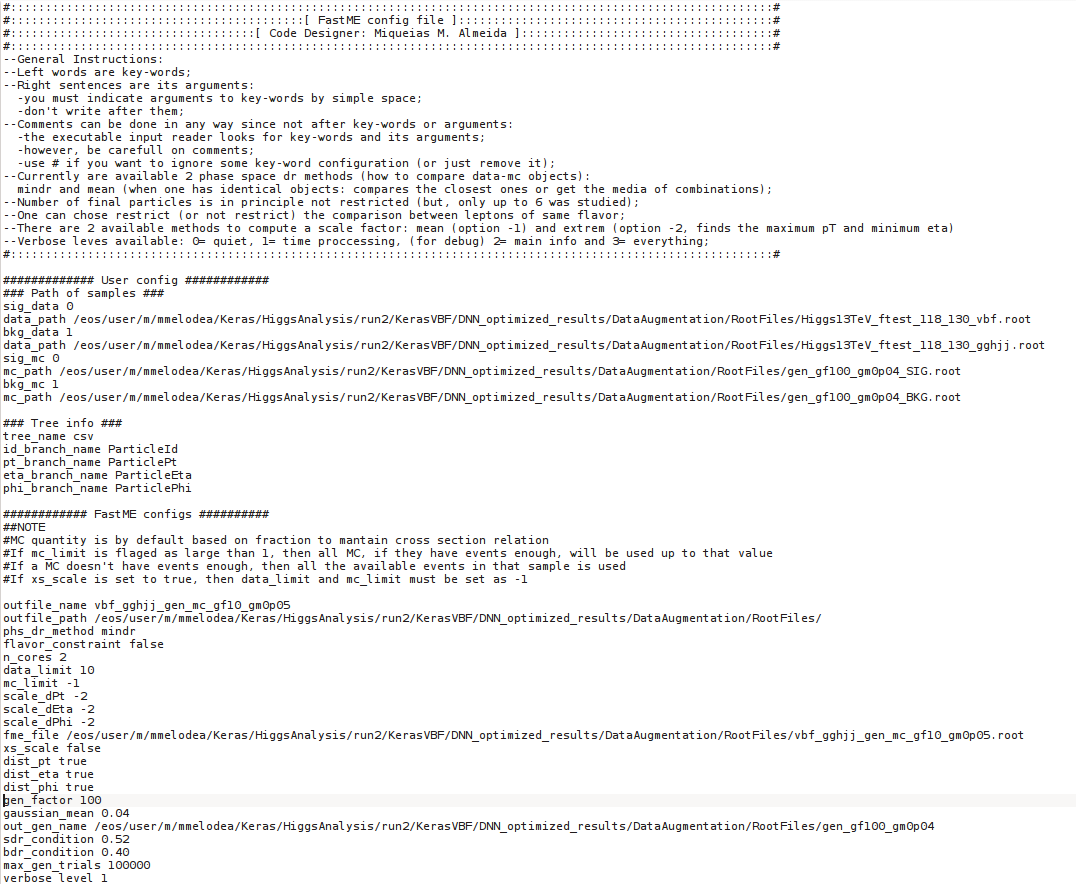
\includegraphics[angle=90,scale=0.7,trim={0cm 0cm 0cm 0cm},clip]{AppendixFastME/figs/fme_config_card}
\source{The AUTHOR, 2015.}
\label{fig:fastme_input_card}
\end{figure}


\subsection{The results provided by the \textit{Fast}ME package}
Once the full analysis in the \textit{Fast}ME has been ran, the user will have some plots which gives the information about the performance of the method on the given dataset. Between these plots the most important are the discriminant distribution for signal and background (it was not developed a feature for superimposing the observed data distribution to the MC). Here is an example of the plots (Fig.~\ref{fig:fms_output_plots}) that are produced by the package. On (a) one sees the discriminant distribution coming from the \textit{Fast}ME method based on the minimum events distance and on (b) it is shown its performance by usage of a ROC curve.

\begin{figure}[htbp]{16cm}
	\caption{Comparison between the two methods developed to define the classification of a event probe. On (a) the discriminant distributions for the minimum distance matching and on (b) its performance.}
	\begin{overpic}
		[width=15cm,height=7cm,trim={0cm 0cm 0cm 2cm},clip]{AppendixFastME/figs/plot_discriminants_roc_distance}
		\put(25,0){(a)}
		\put(75,0){(b)}
	\end{overpic}
	\source{The AUTHOR, 2015.}
	\label{fig:fms_output_plots}
\end{figure}


\subsection{Data Filtering by \textit{Fast}ME}
Another idea that came later for the usage of the \textit{Fast}ME was the particle selection based on the MC. This selection is different from what have been presented so far in the sense that, originally, the \textit{Fast}ME was planed to be used on final data, that is, after a full-selection analysis. However, as the core of the method is based on the idea of matching a given particle from a data event probe to a given particle from a MC event, the straight derivative idea is the possibility of filter out such data probe particles through the same principles. So, the idea here was to test and see how the method works when one has more particles in data than it is expected from the MC. 

In order to test this situation, random values of $p_{T}$, $\eta$ and $\phi$ (constrained within the expected range of such variable) were introduced in the sample of observed events. Here, the tests were done for the case without jets and only the four leptons coming from the Higgs decay have been used (the same samples presented before). The Fig.~\ref{fig:fme_particle_filter} shows how the discriminant behaves under such situation, where it was tested the presence of up to 46 extra objects in the data event (there were always the selected four leptons of the probing event). As one can see, the method is sensitive to the presence of extra particles and its performance decreases fast the number of those particles. But, it seems to work reasonably up to 4 extra particles. Note that in those tests the size of the bank was constrained to 5k. With a larger pattern bank these performances could increase.

\begin{figure}[htbp]{16cm}
\caption{Variation on the \textit{Fast}ME performance due the introduction of extra objects with random properties in the signal and background testing samples. In (a) the variation on the signal and background distributions for the discriminant (based on distance) and in (b) the variation on the ROC curve.}
\subfloat[]{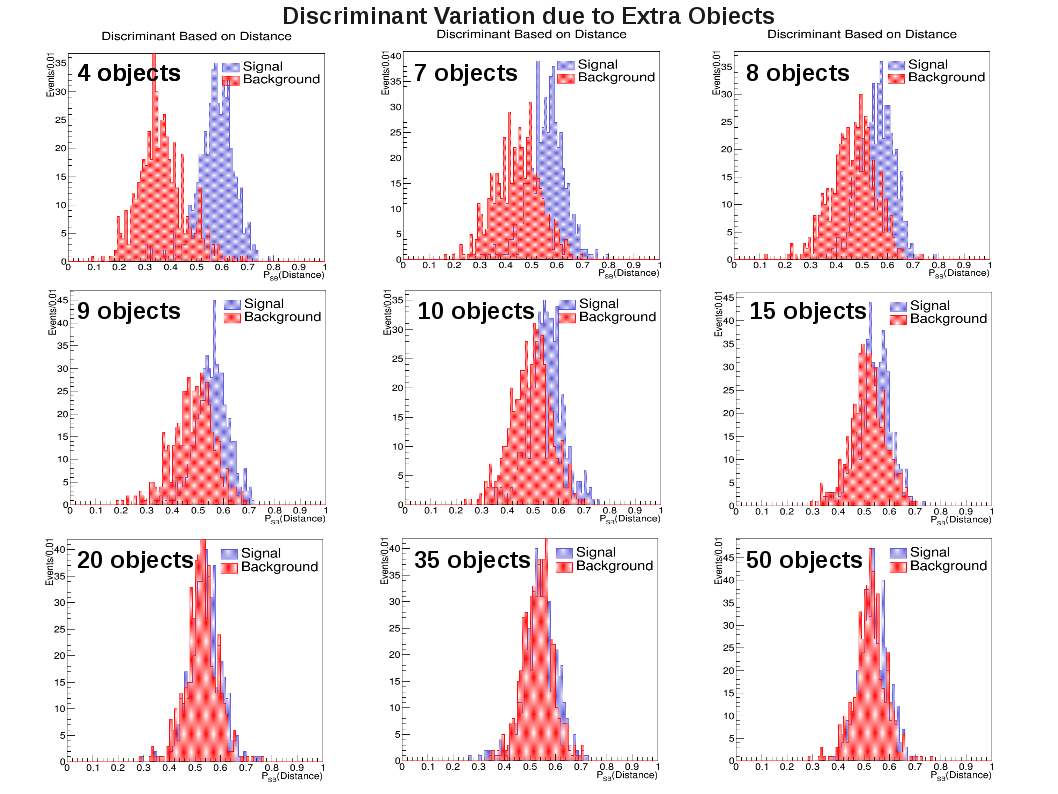
\includegraphics[scale=0.5,trim={0cm 0cm 0cm 1.2cm},clip]{AppendixFastME/figs/discriminant_variation_vs_nextra_objects}}\\
\subfloat[]{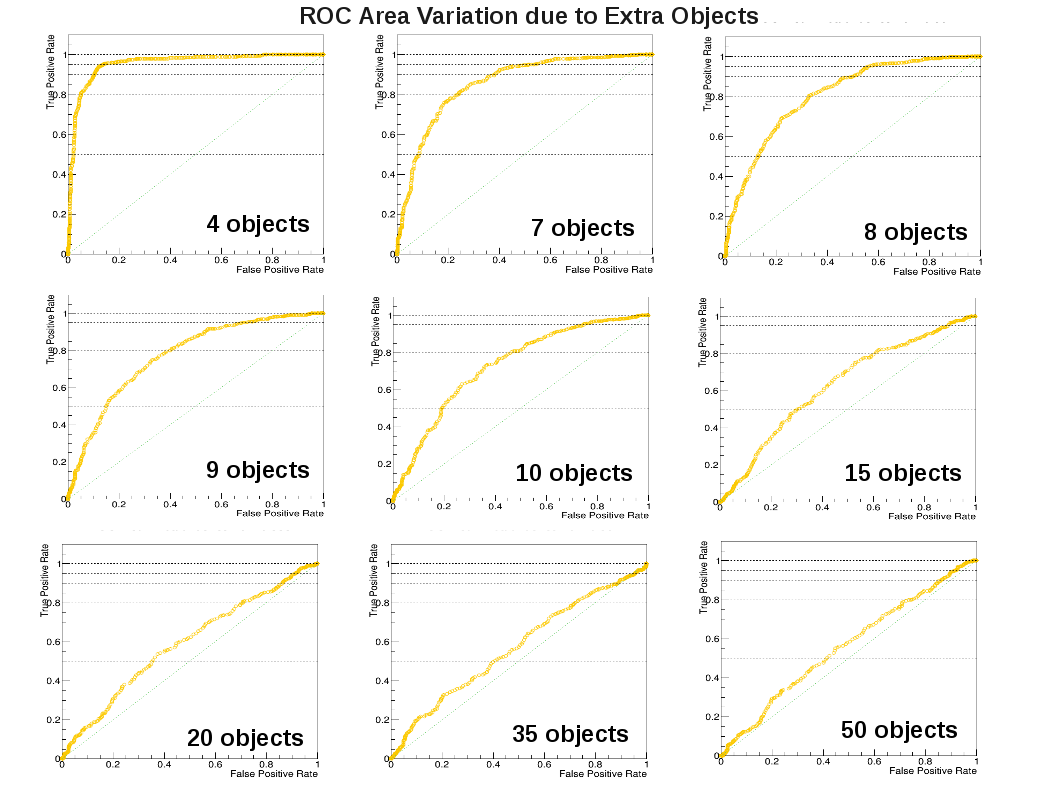
\includegraphics[scale=0.5,trim={0cm 0cm 0cm 0.8cm},clip]{AppendixFastME/figs/roc_variation_vs_nextra_objects}}
\source{The AUTHOR, 2016.}
\label{fig:fme_particle_filter}
\end{figure}


\subsection{The \textit{Fast}ME Applied to qqH vs. ggH}
The final topic of study involving the \textit{Fast}ME was the attempt of VBF discrimination against gluon-fusion. The main subject of the present thesis is the measurement of Higgs VBF production XS. So, it was natural to think about applying the \textit{Fast}ME to the VBF selection. In this case, the inputs were the four leptons and two jets $p_{T}$, $\eta$ and $\phi$. The Fig.~\ref{fig:fme_vbf_ggh} shows the outcome found when trying to discriminate the VBF process against the gluon-fusion. The overlap between the discriminant distributions from each process is visibly large and its performance, as it is shown by the ROC curve, is very low (AUC $\sim 66\%$). Here it is shown only the performance from the method based on the distance, since, as already said on previous sections, this method was the one presenting highest performance.

\begin{figure}[h]{16cm}
\caption{\textit{Fast}ME performance on the discrimination of qqH against ggH using the discriminant based on the distance (left). The area under the ROC curve (right) corresponds to $\sim 66\%$.}
\begin{overpic}
[width=15cm,height=3cm,trim={0cm 0cm 0cm 1cm},clip]{AppendixFastME/figs/ggH_vs_VBF_test}
\put(25,0){(a)}
\put(75,0){(b)}
\end{overpic}
\source{The AUTHOR, 2016.}
\label{fig:fme_vbf_ggh}
\end{figure}
